\makeatletter
\def\input@path{{../DecisionSupportSystems/}}
\makeatother
\documentclass[a4paper,11pt,oneside]{memoir}
% Dokumentklassen sættes til memoir.
% Manual: http://ctan.org/tex-archive/macros/latex/contrib/memoir/memman.pdf
%\documentclass[a4paper,11pt,twoside,openright]{memoir}
\setlrmarginsandblock{*}{2.5cm}{0.75} % højre og venstre 
\setulmarginsandblock{3cm}{*}{1.2} % top og bund 
\checkandfixthelayout[nearest] % specifikt valg af højde algoritme

%Styrer hvordan nye afsnit håndteres
%https://www.sharelatex.com/learn/Paragraph_formatting#Reference_guide
\parindent=1em %Start på nyt afsnit rykkes ind
\parskip=0.5em %Mellemrum mellem afsnit
 
% Danske udtryk (fx figur og tabel) samt dansk orddeling og fonte med
% danske tegn. Hvis LaTeX brokker sig over æ, ø og å skal du udskifte
% "utf8" med "latin1" eller "applemac". 
\usepackage[utf8]{inputenc}
\usepackage[english]{babel}
\usepackage[T1]{fontenc}
\usepackage{mflogo}

%bruges til at fastgøre billeder hvor man vil have dem ved brug af H
\usepackage{float}

%sexy pdf'er
%\usepackage[export]{adjustbox}
\usepackage{pdfpages}
\usepackage{pdflscape}

%Kompakte lister
\usepackage{paralist}
 
% Matematisk udtryk, fede symboler, theoremer og fancy ting (fx kædebrøker)
\usepackage{amsmath,amssymb}
\usepackage{bm}
\usepackage{amsthm}
\usepackage{mathtools}

% Fancy ting med enheder og datatabeller. Læs manualen til pakken
% Manual: http://www.ctan.org/tex-archive/macros/latex/contrib/siunitx/siunitx.pdf
\usepackage{siunitx}
 
%Fancy headers, 
%Manual: https://www.sharelatex.com/learn/Headers_and_footers
\let\footruleskip\undefined
\usepackage{fancyhdr}
\pagestyle{fancy}

 
% Indsættelse af grafik. og man kan rotere tekst in line
\usepackage{graphicx} 
\usepackage{fix-cm} 
\usepackage{soul}
\sodef\an{}{0.13em}{0em}{0em} \sodef\ann{}{0.13em}{0.5em}{0em}
 

%Fancy tabeller.
%\usepackage[table]{xcolor}
\usepackage{multirow}
\usepackage{rotating} %sidewaystables!
\usepackage{longtable} %tables spanning multible pages.
\usepackage{tablefootnote} %for at indstætte fornoter i tabeller.
\usepackage{hhline} %Fixer farvede felter
\usepackage{ltxtable} %Longtabular X
\usepackage{tabularx} %Med dynamisk bredte

%URL fodnoter
\usepackage{url}

% Reaktionsskemaer. Læs manualen for at se eksempler.
% Manual: http://www.ctan.org/tex-archive/macros/latex/contrib/mhchem/mhchem.pdf
\usepackage[version=3]{mhchem}

%Lav chapter clickable og fjern border
\usepackage{hyperref}
\hypersetup{
    colorlinks,
    citecolor=black,
    filecolor=black,
    linkcolor=black,
    urlcolor=black
}

%Table of contents settings
\setsecnumdepth{subsection} % organisational level that receives a numbers
\settocdepth{subsection}   % print table of  for level 3

%Til programkode
\usepackage{listings}
\usepackage{color}

\definecolor{dkgreen}{rgb}{0,0.6,0}
\definecolor{gray}{rgb}{0.5,0.5,0.5}
\definecolor{mauve}{rgb}{0.58,0,0.82}
 
\lstset{ 
  language=C++,                % the language of the code
  basicstyle=\footnotesize,           % the size of the fonts that are used for the code
  numbers=left,                   % where to put the line-numbers
  numberstyle=\tiny\color{gray},  % the style that is used for the line-numbers
  stepnumber=1,                   % the step between two line-numbers. If it's 1, each line 
                                  % will be numbered
  numbersep=5pt,                  % how far the line-numbers are from the code
  backgroundcolor=\color{white},      % choose the background color. You must add \usepackage{color}
  showspaces=false,               % show spaces adding particular underscores
  showstringspaces=false,         % underline spaces within strings
  showtabs=false,                 % show tabs within strings adding particular underscores
  frame=single,                   % adds a frame around the code
  rulecolor=\color{black},        % if not set, the frame-color may be changed on line-breaks within not-black text (e.g. commens (green here))
  tabsize=2,                      % sets default tabsize to 2 spaces
  captionpos=b,                   % sets the caption-position to bottom
  breaklines=true,                % sets automatic line breaking
  breakatwhitespace=false,        % sets if automatic breaks should only happen at whitespace
  title=\lstname,                   % show the filename of files included with \lstinputlisting;
                                  % also try caption instead of title
  keywordstyle=\color{blue},          % keyword style
  commentstyle=\color{dkgreen},       % comment style
  stringstyle=\color{mauve},         % string literal style
  escapeinside={\%*}{*)},            % if you want to add LaTeX within your code
  morekeywords={*,...},               % if you want to add more keywords to the set
  rangeprefix=//----------,			%Used for sexy code includes
  rangesuffix=----------,			%---||---
  includerangemarker=false,			%---||---
  literate=
  {á}{{\'a}}1 {é}{{\'e}}1 {í}{{\'i}}1 {ó}{{\'o}}1 {ú}{{\'u}}1
  {Á}{{\'A}}1 {É}{{\'E}}1 {Í}{{\'I}}1 {Ó}{{\'O}}1 {Ú}{{\'U}}1
  {à}{{\`a}}1 {è}{{\`e}}1 {ì}{{\`i}}1 {ò}{{\`o}}1 {ù}{{\`u}}1
  {À}{{\`A}}1 {È}{{\'E}}1 {Ì}{{\`I}}1 {Ò}{{\`O}}1 {Ù}{{\`U}}1
  {ä}{{\"a}}1 {ë}{{\"e}}1 {ï}{{\"i}}1 {ö}{{\"o}}1 {ü}{{\"u}}1
  {Ä}{{\"A}}1 {Ë}{{\"E}}1 {Ï}{{\"I}}1 {Ö}{{\"O}}1 {Ü}{{\"U}}1
  {â}{{\^a}}1 {ê}{{\^e}}1 {î}{{\^i}}1 {ô}{{\^o}}1 {û}{{\^u}}1
  {Â}{{\^A}}1 {Ê}{{\^E}}1 {Î}{{\^I}}1 {Ô}{{\^O}}1 {Û}{{\^U}}1
  {œ}{{\oe}}1 {Œ}{{\OE}}1 {æ}{{\ae}}1 {Æ}{{\AE}}1 {ß}{{\ss}}1
  {ç}{{\c c}}1 {Ç}{{\c C}}1 {ø}{{\o}}1 {å}{{\r a}}1 {Å}{{\r A}}1
  {€}{{\EUR}}1 {£}{{\pounds}}1
}

%Til at udregne forskel mellem sider, brug \pagedifference{A}{B} mellem to labels A og B.
\usepackage{refcount}
\newcommand{\pagedifference}[2]{%
  \number\numexpr\getpagerefnumber{#2}-\getpagerefnumber{#1}\relax}
 
%Til at lave referencer med:
\usepackage{cite}

%Til at lave eksterne \ref til \labels
\usepackage{xr}

%Til at lave \Beam (DC symbol)
\usepackage{marvosym}

%Forsøg på nice lister i tabeller
\usepackage[shortlabels]{enumitem}

\newenvironment{packed_enum}{
\begin{enumerate}[1., topsep=0pt, nosep, partopsep=0pt, itemsep=0pt, parsep=0pt]
}{\end{enumerate}}

\newenvironment{packed_item}{
\begin{itemize}[•, topsep=0pt, nosep, partopsep=0pt, itemsep=0pt, parsep=0pt]
}{\end{itemize}}

%Lækker kommando til at skrive I2C flot uden at bruge \textsuperscript hver gang:
\newcommand*{\IIC}{\texorpdfstring{I\textsuperscript{2}C }{I2C}}

%Lækker kommando til ref. -> \ref{input} \nameref{input} på side \pageref{input}
\newcommand*{\myRef}[1] {\ref{#1} \nameref{#1} på side \pageref{#1}}

%Lorem ipsum
\usepackage{lipsum}


\usepackage{longtable}
\usepackage{array} % for extrarowheight

%Juicy columntypes - http://tex.stackexchange.com/questions/12703/how-to-create-fixed-width-table-columns-with-text-raggedright-centered-raggedlef
\newcolumntype{L}[1]{>{\raggedright\let\newline\\\arraybackslash\hspace{0pt}}p{#1}}
\newcolumntype{C}[1]{>{\centering\let\newline\\\arraybackslash\hspace{0pt}}p{#1}}
\newcolumntype{R}[1]{>{\raggedleft\let\newline\\\arraybackslash\hspace{0pt}}p{#1}}
\newcolumntype{Z}{>{\raggedright\arraybackslash}X}

%Dejlig kommando til at få nye kapitler på højre side
\newcommand*\cleartorightpage{%
	\clearpage
 	\checkoddpage
	\ifoddpage
  		%do nothing
	\else
		\thispagestyle{empty}
		\mbox{}
 		\clearpage
	\fi
}


%Hacky løsning til at ordne indholdsfortegnelsen.. Why memoir class.. WHY??!
\renewcommand*{\cftdotsep}{1}
\setpnumwidth{3em}
\setrmarg{4em}

%Bugfix til Longtables
\makeatletter
\def\LT@start{%
  \let\LT@start\endgraf
  \endgraf\penalty\z@\vskip\LTpre
  \dimen@\pagetotal
  \advance\dimen@ \ht\ifvoid\LT@firsthead\LT@head\else\LT@firsthead\fi
  \advance\dimen@ \dp\ifvoid\LT@firsthead\LT@head\else\LT@firsthead\fi
  \advance\dimen@ \ht\LT@foot
  \edef\restore@vbadness{\vbadness\the\vbadness\relax}% (added)
  \vbadness=\@M % (added)
  \dimen@ii\vfuzz
  \vfuzz\maxdimen
    \setbox\tw@\copy\z@
    \setbox\tw@\vsplit\tw@ to \ht\@arstrutbox
    \setbox\tw@\vbox{\unvbox\tw@}%
  \vfuzz\dimen@ii
  \restore@vbadness % (added)
  \advance\dimen@ \ht
        \ifdim\ht\@arstrutbox>\ht\tw@\@arstrutbox\else\tw@\fi
  \advance\dimen@\dp
        \ifdim\dp\@arstrutbox>\dp\tw@\@arstrutbox\else\tw@\fi
  \advance\dimen@ -\pagegoal
  \ifdim \dimen@>\z@\vfil\break\fi
      \global\@colroom\@colht
  \ifvoid\LT@foot\else
    \advance\vsize-\ht\LT@foot
    \global\advance\@colroom-\ht\LT@foot
    \dimen@\pagegoal\advance\dimen@-\ht\LT@foot\pagegoal\dimen@
    \maxdepth\z@
  \fi
  \ifvoid\LT@firsthead\copy\LT@head\else\box\LT@firsthead\fi\nobreak
  \output{\LT@output}%
}
\makeatother

%Debugging
%\overfullrule=2cm
\usepackage{amsmath}
\usepackage{amsfonts}
\usepackage{amssymb}
\title{Decision Support Systems \\ Team 3}
\author{Report \\ Aarhus University, Science and Technology \\ Lector: Christian Fischer Pedersen}
\date{\today}
\begin{document}
\fancyhf{} %Clear all header/footers
\frontmatter
\maketitle
\vfill

%\begin{figure}
%	\centering
%	\includegraphics[scale=1, trim=125 110 120 650, clip=true]{../fig/forside_rapport_underskrevet}
%\end{figure}

\begin{table} [h]
	\centering
	\begin{tabular}{|l|r|l|}
	\hline 
	\textbf{Name} 				& \textbf{Study number} & \textbf{Signature~~~~~~~~~~~~~~~~~~~~} 	\\ \hline
	David Jensen 				& 11229 	& \\ && 												\\ \hline
	Henrik Bagger Jensen 		& 201304157 & \\ && 												\\ \hline
	Ólafur Dagur Skúlason 		& IY11249	& \\ && 												\\ \hline
	Titas Urbonas 				& 201700321 & \\ && 												\\ \hline
	Christian M. Lillelund 		& 201408354 & \\ && 												\\ \hline
	\end{tabular}
\end{table}

\clearpage
\pagestyle{plain}

\tableofcontents

\vfill

\mainmatter
\pagestyle{fancy}
\fancyhf{} %Clear all header/footers
\fancyhead[R]{Team No. 3}
\fancyhead[C]{\nouppercase{\leftmark}}
\fancyhead[L]{Aarhus University}
\fancyfoot[C]{\nouppercase{\rightmark}}
\fancyfoot[R]{\thepage}

\chapter{Introduction} \label{ch:introduction}

This document will cover the concepts covered in the course Decision Support Systems and is segmented by lecture topic covering a broader catagory of supervised or unsupervised learning. This report is intended to give an overview of the methods discussed during lectures, but not to be a definitive guide to machine learning methods.

Decision support systems are a field of study that focuses on using statistical models to provide understanding of the context that is free of cognitive biases and sufficiently numerical in nature to allow computer agents to use them as the basis for making decisions despite uncertainty. As problems become more complex, the capacity of humans to gain oversight and understanding of the situation drops, and computers start needing more complex heuristics to make decisions. In both cases relying on humans adds weakness to the solution as they tend to use few simple heuristics to make decisions, which often leads to severe and often repeated errors\footnote{\cite{Tversky1975}}.

When it comes to AI and machine learning, decision support systems can be applied to allow the machine to handle uncertainty in a systematic manner. The machine will then be able to create highly complex decision models based on available data, in ways that no human programmer could manage. Many of the topics covered in the course rely heavily on the application of statistical methods for producing their results. As such many of the fallacies an author might make with statistics also applies to machine learning methods, as the foundation is the actual statistical measurement techniques. If a statistics model is poorly designed by an individual, it might as well perform badly in a computer setting.

This could also lead to illusory correlation, where a certain association between variables in a model correlate with each-other, thus a causation is assumed if one blindly trusts the statistical model. Statistics and machine learning are extremely useful tools and will continue to see use in modern society and technology, but it is important to keep in mind the mathematics behind and use common sense when evaluating the results.
								    \clearpage
\chapter{Regression} \label{ch:regression}

This chapter details the work of LAB exercise 3.6.2, 3.6.3, 4.6.1 and 4.6.2 from "An Introduction to Statistical Learning". It starts by recapitulating the theory behind linear regressions, both simple and multiple, then proceeds to describe the accompanied LAB exercises and conclude on their findings.

\section{Multiple Linear Regression}\label{sc:multipleLinearRegression}

\subsection{Theory}

Basic theory for simple and multiple lin regs here. From the slides or book.

Simple Linear Regression is used to make linear models of data. It has a response Y on the basis of a single predictor variable X. We can write it as
$Y = \beta_0 + \beta_1 X_1 + \epsilon_i$.
$ \beta_0 + \beta_1 $ are unknown and to get a response, we must use data to estimate the coefficients.
$(x_1, y_1), (x_2, y_2), . . . , (x_n, y_n)$
represent n observation pairs, each of which consists of a measurement of X and a measurement of Y. The drawback of this method is that only a single predictor variable is used and often have more.
 In cases where we want examined the relationship between multiple predictor variables we use Multiple Linear Regression. The model takes the following form $Y = \beta_0 + \beta_1 X_1 + ... + \beta_n X_n + \epsilon_i$

To obtain the Coefficients in the model we use the least squares method to minimize the sum of squared residuals. We pick $\beta_0, \beta_1, ... \beta_p$ to to minimize the sum of squared residuals.
$$RSS = \sum (y - \hat{y})^2 = \sum( y_i - \hat{\beta_0} - \hat{\beta_1}x_\textit{i}1 + \hat{\beta_2}x_\textit{i}2 - \dots - \hat{\beta_p}x_\textit{i}p )^2$$

To evaluated the model we can use RSE (residual standard error)


\subsection{Results}

LAB 3.6.2 + 3.6.3

\subsection{Conclusion}

\subsection{Logistic Regression}\label{sc:logisticRegression}
We sometimes want to classify a response variable that has two classes. Examples of such classes could be being accepted or rejected into school based or the market going up or down. There for our target class Y should be seen as a binary class. Where $0$ suggest Reject(Negative Class) and $1$ suggest Accept(Positive Class).
\subsection{Theory}
So we want to model the probability of the default class. If we are modeling people’s gender as male or female based on their shoe size, then the first class could be male and could be written as the probability of male given a person’s shoe size.
\begin{align}\label{fo:logit}
P(x) = P(gender=male|ShoeSize)
\end{align}
or we could say we are modeling the probability that the input (X) belongs to our default class and that is Y=1.
\begin{align}\label{fo:probability}
P(x) = P(Y=1|X)
\end{align}
We then use the logistic function seen in \ref{fo:LogisticFunction} because it will gives outputs between 0 and 1 for all values of X and will always produce an S-shaped curve.
\begin{align}\label{fo:LogisticFunction}
P(x) = \dfrac{ e^{\beta_0 + \beta_1 X}}{  1 + e^{\beta_0 + \beta_1 X}}
\end{align}
If we move things a little (The $e$ can be removed from one side by adding a natural logarithm $ln$ to the other) we get the following \ref{fo:logit}. Here we can see that it still a linear model, but we are modeling the probabilities on a non-linear scale.
The ratio on the left in the equation is called log odds of the default class. This is calculated as a ratio of the probability of the event divided by the probability of not the event, e.g. 0.5/(1-0.5) which has the odds of 1.
 \begin{align}\label{fo:logit}
\log( \dfrac{ P(X)}{1-P(x)} ) = \beta_0 + \beta_1 X
\end{align}

In a small totally made up example lets pretend we knew $\beta_0 = -10 $ and $ \beta_1 = 0.4 $ and if we use the equations as defined above we can plug in the numbers and find the probability of a male given the shoe size of 24 or put into math $P(x) = P(gender=male|ShoeSize=24)$ and therefor $P(x) = \dfrac{ e^{-10 + 0.4*24}}{1 + e^{-10 + 0.4*24}} = 0.40$ this would mean that the there is a 40\% the person is a male. But we want to set a threshold for our binary classify and that could be something like $0$ if $p(male) < 0.5$ and $1$ if $ p(male) >= 0.5$

\textit{\textbf{\underline{We could add Maximum likelihood estimation??????? that is how it knows beta}}}

\subsection{Results}
In lab 4.6.1 + 4.6.2 we look at stock market data and we will try to predict if the market goes up or down base on the Daily percentage returns for stock index between 2001 and 2005.
After download the dataset using pandas we display the data to get a sense of it.
\begin{lstlisting}[language=Python]
data.head()
\end{lstlisting}
\begin{Verbatim}[commandchars=\\\{\}]
{\color{outcolor}Out[{\color{outcolor}183}]:}    Year   Lag1   Lag2   Lag3   Lag4   Lag5  Volume  Today Direction
1  2001  0.381 -0.192 -2.624 -1.055  5.010  1.1913  0.959        Up
\end{Verbatim}
Because the classifier only works with digits we need to change the Today Direction column into a number and split the data set into a y and X.
\begin{lstlisting}[language=Python]
y, X = dmatrices('Direction~Lag1+Lag2+Lag3+Lag4+Lag5+Volume', data, return_type = 'dataframe')
\end{lstlisting}
Now that we have y and X we can now use the statsmodels library to create a logistic regression and fit the model. Here we also instruct the api to assign Direction[Up] as a 1 thereby also assign 0 as Direction[Down].
\begin{lstlisting}[language=Python]
logit = sm.GLM(y.iloc[:,1],X, family=sm.families.Binomial())
result = logit.fit() # fit the model
\end{lstlisting}

%Now the model is fitted. We can see detailed infomation about our model.
%\begin{lstlisting}
%print (result.summary())
%									--omitted--
%               coef       std err     z          P>|z|      [0.025      0.975]
%------------------------------------------------------------------------------
%Intercept     -0.1260      0.241     -0.523      0.601      -0.598       0.346
%Lag1          -0.0731      0.050     -1.457      0.145      -0.171       0.025
%									--omitted--
%\end{lstlisting}
%A negative for the Lag1 coefficient tell us that if the market had a positive return yesterday, then it is less likely to go up today. But because the P value kind of big still there is no real evidence of good association between Lag1 and Direction.

To get the accuracy of our model we take the mean of data we predicted correctly model hence it only predicted the movement of the market 52.2\% of the time.
\begin{lstlisting}[language=Python]
np.mean(y.iloc[:,1].values == predict_label.iloc[:,0].values) # to get accuracy
0.52159999999999995
\end{lstlisting}
To get better accuracy we will split the dataset into a training set with data before and a test set with data after 2015. This is to get a error rate that matches better with a real serniario where the future is unknown. and try to predict again.

\begin{lstlisting}[language=Python]
Smarket_2005 = data.query('Year >= 2005')
Smarket_train = data.query('Year < 2005')
y_train, X_train = dmatrices('omitted', Smarket_train, return_type = 'dataframe')
y_test, X_test = dmatrices('omitted', Smarket_2005, return_type = 'dataframe')
logit = sm.GLM(y_train.iloc[:,1], X_train, family=sm.families.Binomial())
\end{lstlisting}

Now that our model have been trained we can view detailed information about the fit. A negative for the Lag1 coefficient tell us that if the market had a positive return yesterday, then it is less likely to go up today. But because the P value kind of big still there is no real evidence of good association between Lag1 and Direction.

\begin{lstlisting}[language=Python]
print( logit.fit().summary())
                 Generalized Linear Model Regression Results                  
								--omitted--
				 coef    std err          z      P>|z|      [0.025      0.975]
------------------------------------------------------------------------------
Intercept      0.1912      0.334      0.573      0.567      -0.463       0.845
Lag1          -0.0542      0.052     -1.046      0.295      -0.156       0.047
Lag2          -0.0458      0.052     -0.884      0.377      -0.147       0.056
Lag3           0.0072      0.052      0.139      0.889      -0.094       0.108
Lag4           0.0064      0.052      0.125      0.901      -0.095       0.108
Lag5          -0.0042      0.051     -0.083      0.934      -0.104       0.096
Volume        -0.1163      0.240     -0.485      0.628      -0.586       0.353
==============================================================================
\end{lstlisting}


\begin{lstlisting}[language=Python]
np.mean(y_test.iloc[:,1].reset_index(drop=True)==predict_label.iloc[:,0].reset_index(drop=True))
0.48015873015873017
\end{lstlisting}

The error is still $1 - 0.48 = 0.52$. So it's not that much better then random coin flipping. As we saw earlier our p-values in our model was quit high for Lag3 to Lag5 so by retraining the model without them. This should lead to a more efficient model. 
\begin{lstlisting}[language=Python]
y_train, X_train = dmatrices('Direction~Lag1+Lag2', Smarket_train, return_type = 'dataframe')
y_test, X_test = dmatrices('Direction~Lag1+Lag2', Smarket_2005, return_type = 'dataframe')
preds = logit.fit().predict(X_test)
--omitted--
np.mean(y_test.iloc[:,1].reset_index(drop=True)==predict_label.iloc[:,0].reset_index(drop=True))
0.44047619047619047
\end{lstlisting}
Because 1 - 0.44 = 0.56 there is a 0.56 chance of an error. Hence is shows that there is a 56\% chance that the market should go up on days when the model predict it should. But the dataset is really too small to show if it is trend or just random chance.

\subsection{Conclusion}
Logistic Regression is a good classifier when we what to classify data. But sometimes want to classify a response variable that has more than two classes. This is where discriminant Classification analysis, is good choice for multiple-class classification.
										\clearpage
\chapter{Discriminant Analysis} \label{ch:linearDiscriminantAnalysis}

\section{Linear Discriminant Analysis}
Using Linear Discriminant Analysis we can overcome several problems with Logistic regression {  !!ref bog side 138!! }. When the classes are well-separated, the parameter estimates for the
logistic regression model are unstable. If our sample size is small and the distribution of the predictors X is a normal distribution in each of the classes, the linear discriminant model is again more better than the logistic regression model.
\subsection{Theory}
Before we start using LDA there is a  assumption about the data it operates on. Each of the predictors should be normal distributed for this to work properly. We see the formula used by LDA shown in \ref{fo:BayesTheorem}. Where $\pi_k$ is the prior probability that a randomly selected obsivation comes from the $k$th class. $f_k(x)$ is the probability density function of X for an observation that comes from the $k$th class. If the function is large then there is a high probability that an observation in the $k$th class.

\begin{align}\label{fo:BayesTheorem}
Pr(Y=k|X=x) = \frac{\pi_k f_k(x)}{ \sum_{l=1}^{k}\pi_l f_l(x) }
\end{align}

If we as a example choose to only use one predictor and we would like to obtain the estimate for $f_k(x)$ that we can use in \ref{fo:BayesTheorem} If we assume that $f_k(x)$ is normal distribution it looks like this

\begin{align}\label{fo:BayesTheorem}
Pr(Y=k|X=x) = \frac{\pi_k f_k(x)}{ \sum_{l=1}^{k}\pi_l f_l(x) }
\end{align}

$
\frac{1}{\sqrt{2\pi\sigma_k)}}\exp{}
$

\subsection{Results}
In lab 4.6.3 We use Linear Discriminant Analysis. As we did in lab XXXX we split the data into before and after 2015 and then make training and testing data. Now that we have that out of the way it's time to import the Linear Discriminant Analysis from scikit-learn.
\begin{lstlisting}[language=Python]
from sklearn.discriminant_analysis import LinearDiscriminantAnalysis as LDA
\end{lstlisting}

Now the training process can begin.

\begin{lstlisting}[language=Python]
sklearn_lda = LDA(n_components=2) #creating a LDA object

lda = sklearn_lda.fit(X_train.iloc[:,1:3], y_train.iloc[:,1]) #learning the projection matrix

X_lda = lda.transform(X_train.iloc[:,1:3]) #using the model to project X. Project data to maximize class separation.

X_labels = lda.predict(X_train.iloc[:,1:3]) #gives you the predicted label for each sample

X_prob = lda.predict_proba(X_train.iloc[:,1:3]) #the probability of each sample to belong to each class
\end{lstlisting}

Now that the model have been fitted we will look at the coefficients of the model for Lag1 and Lag2.

\begin{lstlisting}[language=Python]
lda.coef_
array([[-0.05544078, -0.0443452 ]])
\end{lstlisting}

Now we will look at the priors. Therefor we can see that. $$ \hat{ \pi }_1 = -0.05544078  \hat{ \pi }_2 = -0.0443452 $$ 
\begin{lstlisting}[language=Python]
lda.priors_
array([ 0.49198397,  0.50801603])
\end{lstlisting}

Testing step. Now we will test out model using the data.
\begin{lstlisting}[language=Python]
X_test_labels=lda.predict(X_test.iloc[:,1:3])
X_test_prob = lda.predict_proba(X_test.iloc[:,1:3])
\end{lstlisting}

To Get the accuracy of the test set. We use the following command.

\begin{lstlisting}[language=Python]
np.mean(y_test.iloc[:,1]==X_test_labels)
0.55952380952380953
\end{lstlisting}

Let's change the threshod a bit to see whether we can improve the accuracy. The 2nd column of X\_test\_prob is the probability belongs to UP group. The default value is 0.5, let us first check that.

\begin{lstlisting}[language=Python]
threshold = 0.5 
np.mean(y_test.iloc[:,1]==(X_test_prob[:,1]>=threshold))
0.55952380952380953
\end{lstlisting}



\section{Quadratic Discriminant Analysis}
\subsection{Theory}
In some cases, using LDA can be insufficient, since in some cases the data won't be easily deffined as being higher or lower than a linear assumption. In these cases a Quadratic Discriminant Analysis (QDA) can be sufficient. Different from the LDA, the QDA results in a non-linear assumption. The math behind it is given in \ref{fo:quadraticDiscriminantAnalysis1} and \ref{fo:quadraticDiscriminantAnalysis2}.

\begin{align}\label{fo:quadraticDiscriminantAnalysis1}
\delta_k(x) &= - \frac{1}{2} (x - \mu_k)^T \Sigma_{k}^{-1} (x - \mu_k) - \frac{1}{2} \log|\Sigma_{k}| + \log\pi_k\\
			\label{fo:quadraticDiscriminantAnalysis2}
			&= - \frac{1}{2} x^T \Sigma_{k}^{-1} x + x^T \Sigma_{k}^{-1} \mu_k - \frac{1}{2} \mu_k^T \Sigma_{k}^{-1} \mu_k - \frac{1}{2} \log|\Sigma_{k}| + \log\pi_k
\end{align}

Where $\Sigma_{k}$ is a covariance matrix for the \textit{k}th class. Under this assumption, the Bayes classifier assigns an observation $X = x$ to the class for which $\sigma_k$ is largest.

\subsection{Results}
In lab 4.6.4 Quadratic Discriminant Analysis. We split our data as in lab XXXX. We split the data into before and after 2015 and then make training and testing data. After the data is ready we can import the Quadrat Discriminant Analysis from scikit-learn.
\begin{lstlisting}[language=Python]
import sklearn.discriminant_analysis
from sklearn.discriminant_analysis import QuadraticDiscriminantAnalysis
\end{lstlisting}
The training process. Please note we will only use Lag1 and Lag2. Hint iloc[:,1:3] is a way to get first and the second column of data frame.
\begin{lstlisting}[language=Python]
sklearn_qda = QuadraticDiscriminantAnalysis(priors=None,store_covariance=True) #creating a QDA object
qda = sklearn_qda.fit(X_train.iloc[:,1:3], y_train.iloc[:,1]) #learning the projection matrix
X_labels = qda.predict(X_train.iloc[:,1:3]) #gives you the predicted label for each sample
X_prob = qda.predict_proba(X_train.iloc[:,1:3]) #the probability of each sample to belong to each class
\end{lstlisting}
Testing step. Now we will test out model using the data.
\begin{lstlisting}[language=Python]
X_test_labels = qda.predict(X_test.iloc[:,1:3])
X_test_prob   = qda.predict_proba(X_test.iloc[:,1:3])
np.mean(y_test.iloc[:,1]==X_test_labels)
0.59920634920634919
\end{lstlisting}
The QDA predictions are accurate almost 60\% of the time. And we didn't even use all the data to fit the model, because the 2005 data was not used to fit the model. The stock market is pretty hard to model accurately.
This shows that the Quadrat Discriminant Analysis seem to capture the relationship more accurately than the Linear Discriminant Analysis. The output contains the group means. But it does not contain the coefficients of the linear discriminants, because the QDA classifier involves a quadratic, rather than a linear, function of the predictors.

\begin{lstlisting}[language=Python]
qda.means_
array([[ 0.04279022,  0.03389409],
[-0.03954635, -0.03132544]])
\end{lstlisting}
In table format
\begin{longtable}[]{@{}lll@{}}
	\toprule
	& Lag1 & Lag2\tabularnewline
	\midrule
	\endhead
	Down & 0.04279022 & 0.03389409\tabularnewline
	Up & -0.03954635 & -0.03132544\tabularnewline
	\bottomrule
\end{longtable}

\section{K-nearest neighbors}
					\clearpage
\chapter{Resampling Methods}
\section {Bias Variance trade off}
The Bias variance trade off is an important part of modelling and if not done right accuracy of the model will not perform well. We would like a model that that capture the structure of the data but also works well on unseen data and we can't get both. A model with high variance represent the training data well, but are at risk of overfitting hence also capturing the noise in training data. On the other hand models with high bias produce simpler models underfit their training data therefore failing to capture structure of the data.

\begin{figure}[h]
	\centering
	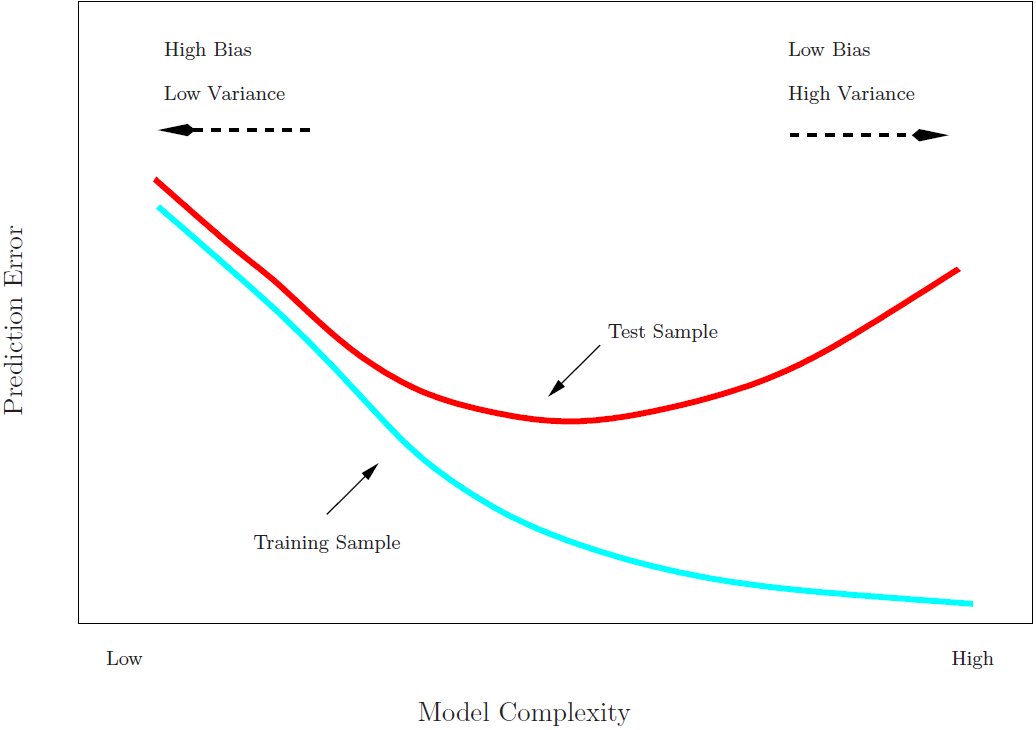
\includegraphics[width=0.5\linewidth]{crossValidation/biasVariance}
	\caption{Bias Variance trade off}
	\label{fig:biasvariance}
\end{figure}


\section{Cross Validation} \label{sc:crossValidation}
Cross validation is a technique for model validation. A model is normally trained on parts of a dataset and later another part of the dataset of unknown data will be tested against the model. With cross validation the aim is to use the the training set in the model in the training to limit problems like overfitting and help gain insight into how the model will behave to a never seen before dataset. There is several options for Cross Validation. The following sections will describe Validation set approach, Leave one out cross validation and K-fold what is the techniques used here.


\section{Validation set approach}
\subsection{Theory}
The Validation set approach works by splitting the data to two parts one is called the training set and the other is called the testing set(validation or hold-out set). An example of the split can be seen on Figure \ref{fig:validationsetapproach}. The model is trained with the training set, after the training is finished the model is tested with the testing set, which the model was not trained on. This test produces a test error, in the form of MSE, which is good for validating the model. The advantage of this method is low computation time, but the results of this method is depended on which data points will end up in the sets. 
\begin{figure}[H]
	\centering
	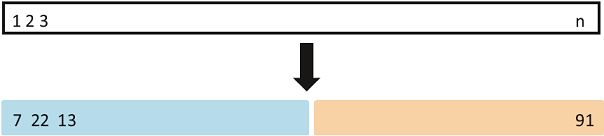
\includegraphics[width=0.4\linewidth]{crossValidation/validationSetApproach}
	\caption{Validation set approach. The entire dataset is split randomly into a training and testing set.}
	\label{fig:validationsetapproach}
\end{figure}

\subsection{Result}
\subsubsection*{LAB 5.3.1}%TODO write full lab
In lab 5.3.1\footnote{Appendix 8 - 5.3.1 The Validation Set Approach} the validation set approach is used to find estimate the test error that result from fitting linear models on the Auto data\footnote{https://raw.github.com/vincentarelbundock/Rdatasets/master/csv/ISLR/Auto.csv} set. First thing is to split the Auto dataset into a training by taking 196 random samples out of the data and use the rest for the testing. We train the model and get the following MSE
\begin{lstlisting}
23.36190289258723
\end{lstlisting}
The MSE looks high so a way to reduce the MSE could be with a polynomial 
\begin{lstlisting}[language=Python]
--------Test Error for 2nd order--------
20.25269085835005
\end{lstlisting}
Cubic regression.
\begin{lstlisting}[language=Python]
--------Test Error for 3rd order--------
20.325609365773605
\end{lstlisting}
By reviewing the results it is clear that the MSE for the models with linear, quadratic, and cubic terms are 23.36, 20.25, and 20.33.


\section {K-fold cross validation}%TODO explain in more detail (give pictures)
\subsection{Theory}
In this type of cross validation the split the data k-subsets and we repeat validation set approach for k times. In each time we take one subest as a test set and other combine are training set. After all copulations we compute average error. The advantage of this method is that all data points are one time in the testing set. The drift of the test is reduced when k is increasing. We can choose the k value, most oftenly k values are 5 or 10 . The disadvantages is that we have to retrain the model k times and the computation time increases. The mathematic formula is below. 
\begin{align}\label{fo:k-fold}
CV_{(K)} = \sum_{k=1}^{K}  \frac {n_{k}}{n}MSE_{(k)}
\end{align}

\subsection{Result}
\subsubsection*{LAB 5.3.3}%TODO write full lab
In the lab 5.3.3 we used K-fold cross validation find the MSE. We are using auto data from the book. In this particular case we are using k = 10. 
\begin{lstlisting}[language=Python]
from sklearn.model_selection import KFold

X = Data["horsepower"].values.reshape(-1,1) 
y = Data["mpg"].values.reshape(-1,1)
kf= KFold()
kf.n_splits = 10
\end{lstlisting}
Now we need to make a loop for all the folds to calculate MSE.   

\begin{lstlisting}[language=Python]
ytests = []
ypreds = []

for train_index, test_index in kf.split(Data):
	X_train, X_test = X[train_index], X[test_index]
	y_train, y_test = y[train_index], y[test_index]

	model = linear_model.LinearRegression()
	model.fit(X = X_train, y = y_train)
	y_pred = model.predict(X_test)  
	ypreds += list(y_pred)
	ytests += list(y_test)
	ms_error = metrics.mean_squared_error(ytests, ypreds)
	print("%.2f" %ms_error, end=" ")
\end{lstlisting}
Out put of the code is:
\begin{lstlisting}[language=Python]
28.35 22.79 24.14 23.95 22.29 21.56 20.92 21.16 26.11 27.42 
\end{lstlisting}
Having all MSE we can choose the best model from the results. or 
\section {Leave one out cross validation}
\subsection{Theory}
The Leave one out cross validation works a lot like Validation set approach but instead of spliting the data set into two subsets of
similar size, a single observation $(x_1, y_1)$ is used for the testing set and the remaining observations ${(x_2, y_2), . . . , (x_n, y_n)}$ make up the training set and repeat this process as seen in Figure \ref{fig:loocv}.
\begin{figure}[H]
	\centering
	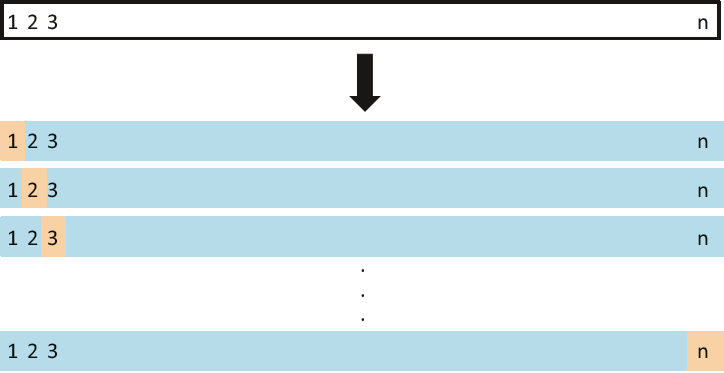
\includegraphics[width=0.5\linewidth]{crossValidation/LOOCV}
	\caption{}
	\label{fig:loocv}
\end{figure}
Repeating this method n times gives n squared errors, $MSE_1, . . . , MSE_n$. The LOOCV estimate for the test MSE is the average of these n test error as shown in Equation \ref{fo:LOOCV}.
\begin{align}\label{fo:LOOCV}
CV_{(n)} = \frac {1}{n} \sum_{k=1}^{K}  (\frac {y_i-\hat{y_i}}{1- h_i})^2
\end{align}
Leave one out cross validation has a some advantages over the validation set approach. It has far less bias. Because in LOOCV repeatedly fit the chosen learning method using training sets that contain n - 1 observations that is nearly as many as are in the entire data set. On the other hand the validation set approach training set is typically around half the size of the original data set hence LOOCV won't overestimate the test error rate as much as the validation set approach would. The LOOCV will also give consistent results because there is no randomness in the training/testing set splits and is usefull when there is limited amount of data.

\subsection{Result}
\subsubsection{LAB 5.3.2}
In lab 5.3.2 the same Auto data as used in the validation Set Approach. Running the iteratively LOOCV process for different fits polynomial regressions for polynomials of 1 to 5 and displaying the associated cross-validation error. The output below shows see a drop in the estimated test MSE between the linear and quadratic fits. But using higher-order polynomials shows no clear improvement.
\begin{lstlisting}[language=Python]
24.23151351792922, 19.24821312448969, 19.334984064109666, 19.42443031091358, 19.0332089609506
\end{lstlisting}
When running the LOOCV a mass increased computing time in the machine has seen and that was expected.
\section{Bootstrap}\label{ch:bootstrap}

A second method for producing additional information from a limited dataset is to use the bootstrap method. It is performed by shaking up the data and plucking out random observations, while allowing for the same observation to be included multiple times, to create a new sample. The process can then be repeated as many times as needed until the desired amount of data becomes available. 

\subsection{Theory}

\iffalse
A good explanation https://stats.stackexchange.com/questions/26088/explaining-to-laypeople-why-bootstrapping-works
\fi

Bootstrapping works on the assumption that distribution parameters are transitive. Such that a random number generated by taking the mean of N samples from a dataset containing N samples, but allowing for replacement, will be equally valid as a random number generated from the original population.

As an example dataset X contains N observations from the original population $\theta$ we resample from X until a new dataset Y with N elements is created. Assuming $\theta$ follows a Gaussian distribution then the mean of Y is a random number generated from the distribution of X which is an estimate of the actual distribution of $\theta$ where each observation is generated from $\theta$. Therefore the mean of Y is an estimated observation from $\theta$.

Assuming we have sufficient data then the estimated distribution can be used for generating a new, more populated, data set without sacrificing much of the quality. As the observed distribution is an estimate of the population distribution, the resulting dataset will have a distribution which is an estimate of the observations.

\iffalse % Olaf: A second attempt at writing this section. Keeping it for review purposes.
Bootstrapping works by resampling the initial data with replacement, until a new data set has been created from the original. The new dataset will then contain a random sample of data with the same distribution as the original, allowing for some deviation in the parameters. By repeating this B times and averaging the distribution parameters over all B samples we get a better estimate of the original population as if we had gotten more observations.

As an example, assuming we have a normally distributed population of N elements then by taking a random resampling from that dataset until a new dataset, also containing N elements, is gained. The mean of that new dataset can then be seen as an estimated new observation from the original population. We then repeat this process B times and in the end we have a new data set of both resampled means and variances. Since both were generated using the original set of observations the set of resamples will also be normally distributed with a mean and variance close to the original population.
\fi

To give an example of how bootstrap creates samples, see Figure \ref{fig:bootstrapDrawWithReplacement}\footnote{\cite{James2013} p. 190}. In the figure random observations are drawn from the estimated population (Original Data(Z)) with replacement. The amount of observations drawn per sample is the same amount as the observations of the estimated population. This creates bins of observations ($Z^{*1}, Z^{*2},\ldots,Z^{*B}$), from the estimated population, from which mean of the data X and Y are both calculated. The result is bootstrap samples ($\hat\alpha^{*1}, \hat\alpha^{*2}, \ldots, \hat\alpha^{*B}$).

\begin{figure}[H]
	\centering
	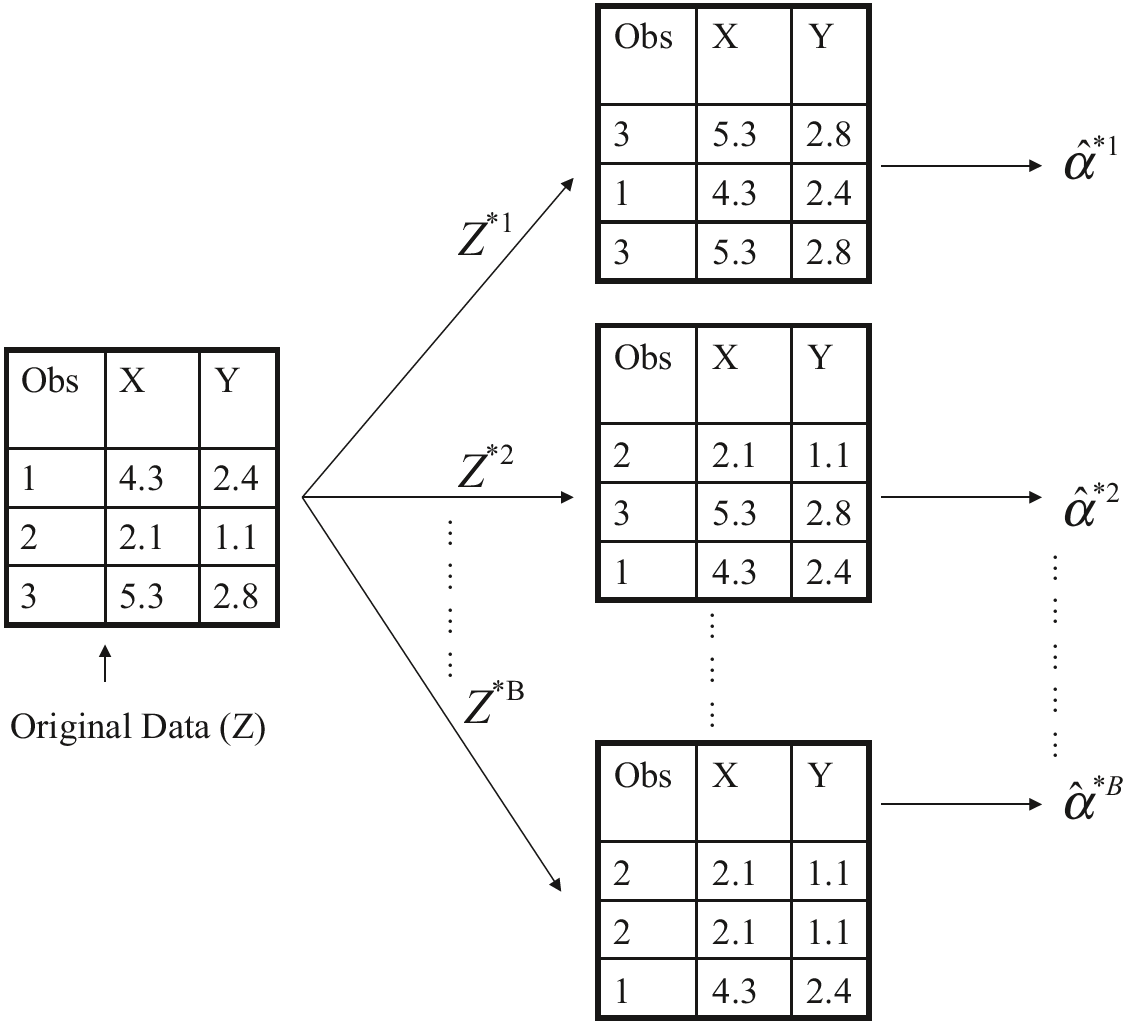
\includegraphics[width=0.5\linewidth]{crossValidation/bootstrapDrawWithReplacement}
	\caption{Bootstrap sample draw, with replacement.}
	\label{fig:bootstrapDrawWithReplacement}
\end{figure}

The standard error of the resampled data can be estimated through the sample standard deviation, as seen in Equation \ref{fo:bootstrapStandardError}. $\hat{\theta}$ denotes the bootstrap data of the estimated population $\theta$. $\hat{\theta_{b}}$ where $b=1,\dots,B$ denotes each bootstrap dataset. $\bar{\theta}$ denotes the mean of the bootstrap data; $\bar{\theta} = \frac{1}{B} \sum_{b=1}^{B}(\hat{\theta_{b}})$.
\begin{align}\label{fo:bootstrapStandardError}
	SE(\hat{\theta}) = \sqrt{\frac{1}{B-1} \sum_{b=1}^{B}(\hat{\theta_{b}} - \bar{\theta})} 
\end{align}

When working with more complex data, for example data that is not independent, but rather dependent on each other can create problems for the resampling methods of bootstrap. The solution to this problem is the Block Bootstrap alternative. Block Bootstrap does the same as the simple bootstrap mentioned earlier in this chapter, however before drawing samples from the estimated population, the data is put into smaller blocks, where the data is independent to each other. The block size is decided upon to maximize the amount of data that reside in a block, as well as minimizing the dependency between data in a single block.

\subsection{Results}
\subsubsection*{LAB 5.3.4}

In lab 5.3.4 on Bootstrap a small data sample is taken and the bootstrapping method is used to increase the data quality. First to examine the process on the Portfolio data set, and then apply the method to the auto data set and review the results for linear and quadratic regression compared to the original.

The resulting mean and error for the intercept and horsepower.
\begin{lstlisting}[language=Python]
original params
  Intercept:  mean:  39.9358610212
  Intercept:  error: 0.717498655555
  horsepower: mean:  -0.157844733354
  horsepower: error: 0.00644550051769
Bootstrapped params
  Intercept:  mean:  39.9805602832
  Intercept:  error: 0.0288069750935
  horsepower: mean:  -0.158352159577
  horsepower: error: 0.000244810973842
\end{lstlisting}

For the linear regression very similar means for both the Intercept and horsepower are found, while the RSE has dropped sharply for both the intercept and horsepower. This shows that the original estimates of the parameters were quite good as most of the error in the estimate can be explained by noise in the data and not $\epsilon_i$ as the regression formula assumes.

For the end of the exercise the same code will be run, but using a quadratic term. This time the fit to the data is very good and we see similar results as the error drops by a factor of $\sim30$.

\begin{lstlisting}[language=Python]
original params
 Intercept:  mean:               56.9000997021
 Intercept:  error:              1.80042680631
 horsepower: mean:               -0.466189629947
 horsepower: error:              0.0311246171196
 np.power(horsepower, 2): mean:  0.00123053610077
 np.power(horsepower, 2): error: 0.00012207586276
Bootstrapped params
 Intercept:  mean:               57.072651342
 Intercept:  error:              0.066630006277
 horsepower: mean:               -0.469465867184
 horsepower: error:              0.00106828698911
 np.power(horsepower, 2): mean:  0.00124365698568
 np.power(horsepower, 2): error: 3.87603834867e-06
\end{lstlisting}



						\clearpage
\chapter{Subset Selection} \label{ch:subsetSelection}							\clearpage
\chapter{Shrinkage Methods} \label{ch:shrinkageMethods}
Before we talked about methods that can be used to select the best subset of predictors. Shrinkage Methods regularizes or penalties the coefficient by shrinking the coefficients towards zero. Using this techniques that can reduce the variance. 

\section{Theory}
\subsection{Vector norm}
A norm is a function that gives a positive length to each vector in a vector space.

\noindent Using the P-norm$ \lVert X \rVert_p = ( \sum_{i=1}^{n}|x_i|^p  )^1/p $ \textbf{ref til wiki Norm(mathematics)}. If we set $ p = 1 $ we get the first norm also called the Manhattan norm. It got it's name because it works in a similar to how a taxi would drive in New York City always in a grid-like route 1 block the east then 2 block to the north. The second norm is called Euclidean distance and that is the distance in a straight line just as a bird would fly. Both norms can be seen visually on Figure \ref{fig:normfirstsecond}.

\begin{figure}[H]
	\centering
	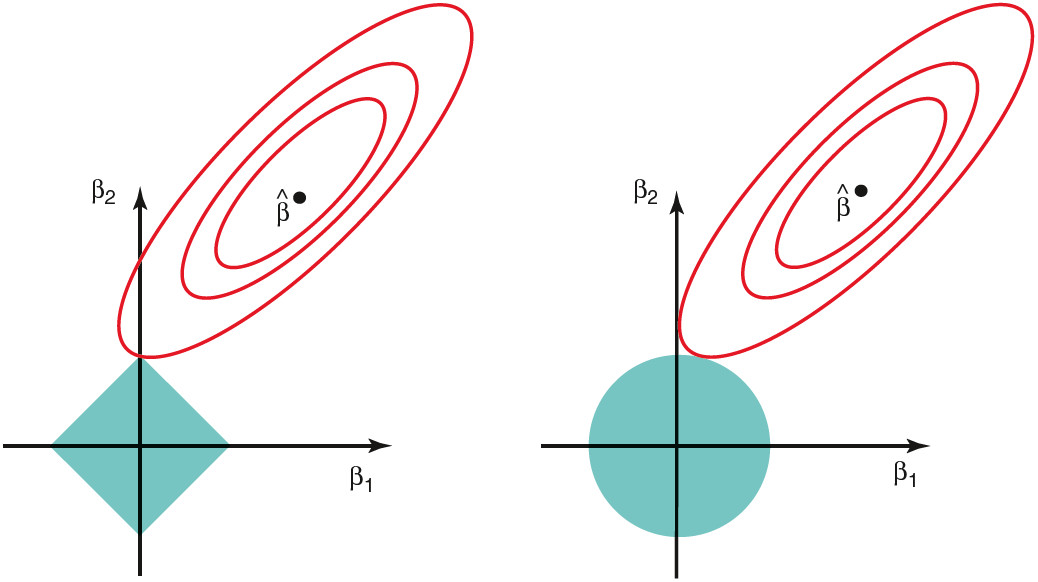
\includegraphics[width=0.6\textwidth]{shrinkageMethods/fig/normsL1_L2.jpg}
	\caption{The red eclipse shows the concurs of ridge (left) and lasso (right) regression. The blue areas are constraint regions for the first and second norm. Notice that lasso intersects the constraint region at an axis, whereas ridge does not.}
	\label{fig:normfirstsecond}
\end{figure}

\subsection{Ridge regression}
The formula for Ridge regression can be seen in \ref{fo:RidgeRegression}. In blue we have the residual sum of square (RSS) term and in red we have the regularize or penalty term. The penalty term is small when $\beta_1, . ,\beta_p$ are close to zero and it has the effect of shrinking or penalizing the estimates of the coefficients $\beta_j$ towards zero. $\lambda$ also called a tuning parameter decides how much impact the two terms get. If $\lambda = 0$ then we will only get least squares estimates, but as $ \lambda \to \infty$ the penalty terms influence will increase and therefore the coefficients will approach zero. This means that the results will be different depending on the chosen $\lambda$ so for getting a good result picking the right $\lambda$ is important.

\noindent The penalty term only apply to the slope, not the intercept. $\lambda$ in in \ref{fo:RidgeRegression} control the degree of penalty.
\begin{align}\label{fo:RidgeRegression}
\color{blue} \sum_{i=1}^{n} ( y_i - \beta_0 - \sum_{j=1}^{p} \beta_j x_i,j )^2 \color{black} + \color{red} \lambda \sum_{j=1}^{p} \beta^2_j 
\end{align}
The reason to Ridge regression over least squares is found in the bias-variance
trade-off. This is because as our $\lambda$ gets bigger the complexity of the ridge regression fit decreases leading to less variance but more bias.

\subsection{The lasso regression}
The formula for least absolute shrinkage and selection operator, also called Lasso, can be seen in figure \ref{foTheLasso}. The blue part of the equation is the RSS (the ) and the red part is the penalty. The lasso regression has a advantage over Ridge regression because of the way the penalty term works. In Ridge it will include all $p_i$ predictors because the $\lambda \sum_{j=1}^{p} \beta^2_j$ only shrink all of the coefficients towards zero but not setting any of them to zero. In lasso we use as E \_ 1 norm of a coefficient vector $\beta$ is given by $ \lVert \beta_1 \rVert = \sum | \beta_j |$ which makes some of the coefficient estimates to be exactly zero when the tuning parameter $\lambda$ is large enough.
\begin{align}\label{fo:TheLasso}
\color{blue} \sum_{i=1}^{n} ( y_i - \beta_0 - \sum_{j=1}^{p} \beta_j x_i,j )^2 \color{black} +  \color{red} \lambda \sum_{j=1}^{p} |\beta_j|
\end{align}
Because the lasso regression removes some of the coefficients, lasso models are generally easier to understand than Ridge regression ones because they are  more sparse with a reduced complexity. Lasso models involve only a subset of the variables. As before selecting a good $\lambda$ is again important here.

\subsection{Comparing ridge and lasso regression}

From equations \ref{fo:RidgeRegression} and \ref{fo:TheLasso} we see that a Lasso regression model could potentially end up with less variables than Ridge regression, since the coefficients can be forced to equal zero, because of the $\ell_1$ penalty. This is called sparsity. You would typically use Ridge regression to prevent over-fitting, since it keeps all features, but can prove less useful with a large number of features (\textit{p} > \textit{n}) On the other hand, Lasso is useful when you have many features and provides you with a more sparse model that could prove a computational advantage. In terms of prediction error, Ridge regression generally performs better in terms of bias, variance and MSE when the predictors are related to the response, that is none of the true coefficients are zero. However if the response is just a subset of the original predictors, we tend to get better results with Lasso regression.

\section{Results}
In lab 6.6.1 we use Ridge Regression on the hitters dataset. We use scikit-lean and their implmeation. After loading the data we found that some players had missing salary, therefor these were dropped. The data also contained some string values and usingf'' pandas we have converted them into dummy variables.  
\begin{figure}[H]
	\centering
	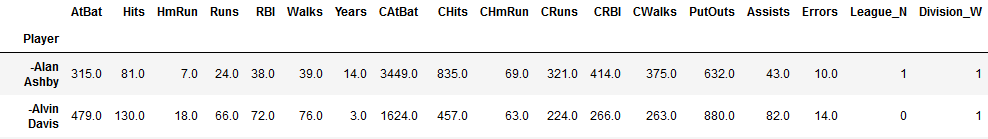
\includegraphics[width=0.8\textwidth]{shrinkageMethods/fig/data.png}
	\caption{The data after removing missing values and making strings into dummy variables }
	\label{fig:normfirstsecond}
\end{figure}
Then we split our data into a training and test set and we try to run Ridge Regression with a alpha of 4 and display our mean squared error.
\begin{lstlisting}[language=Python]
ridge = Ridge(alpha=4)
ridge.fit(X_train, y_train)
result = ridge.predict(X_test)
metrics.mean_squared_error(y_test, result)
134512.83820473132
\end{lstlisting}
After that we display some of the coefficients.
\begin{lstlisting}[language=Python]
pd.Series(ridge.coef_.flatten(), index=X.columns)
AtBat          -2.185390
Hits            7.392346
HmRun          -2.666724
\end{lstlisting}
If we run the same code again but with a alpha that is very large $10^10$ then are coefficients get even smaller.
\begin{lstlisting}[language=Python]
AtBat          5.135079e-04
Hits           1.771301e-04
HmRun          2.568334e-05
-- omitted --
\end{lstlisting}
And our MSE also gets even higher.
\begin{lstlisting}[language=Python]
211698.60251243794
\end{lstlisting}
As discussed in the theory and see just before picking the right alpha part of this is important. We will now use cross validation to pick the best alpha using scikit learn's RidgeCV. That is Ridge regression with built-in cross-validation.
\begin{lstlisting}[language=Python]
alphas = 10**np.linspace(100,-4,1000)
ridgecv = RidgeCV(alphas=alphas, scoring='neg_mean_squared_error')
ridgecv.fit(scale(X_train), y_train)
ridgecv.alpha_
2.3570694139967037
\end{lstlisting}
Now we will use the alpha we found using  cross validation and check our result.
\begin{lstlisting}[language=Python]
ridge = Ridge(2.3570694139967037)
ridge.fit(X_train, y_train)
result = ridge.predict(X_test)
metrics.mean_squared_error(y_test, result)
134355.75204499933
\end{lstlisting}
In lab 6.6.2 we use The Lasso and the same steps to prepere the dataset as before. We need to select the best alpha and to do this we use LassoCV that has cross validation built ind.
\begin{lstlisting}[language=Python]
alphas = 10**np.linspace(100,-20,100)
lassoCV = LassoCV(alphas=alphas)
lassoCV.fit(X_train, y_train)
lassoCV.alpha_
1072.2672220103254
\end{lstlisting}
As we can see some of the coefficients here are zero just as we described in the theory section.
\begin{lstlisting}[language=Python]
pd.Series(lassoCV.coef_.flatten(), index=X.columns)
AtBat          0.729684
Hits           0.000000
HmRun         -0.000000
Runs           0.000000
-- omitted --
\end{lstlisting}






							\clearpage
\chapter{Clustering Methods} \label{ch:clusteringMethods}
So far the report covered only at supervised learning, where a correct pair of input and output variables ($X$ and $y$) were given to train the model and verify our results. An analog to this is a teacher supervising the learning. The teacher have the correct answers and the algorithm iteratively makes predictions on our data and is corrected by the teacher. In unsupervised learning we do not have a output variable $y$, only the features $X_1$, $X_2$,...,$X_p$. This compel us to not look at predictions, but rather interesting things about the observed measurements and possibly discover subgroups in the data. The clustering was used as a technique to perform unsupervised learning. This chapter will cover K-means and hierarchical clustering.

\section{K-means Clustering}
\subsection{Theory}
The way that K-means clustering works is that there is a $C_1,...,C_k$ sets that contains part of the observations. These sets needs to satisfy two properties.
\begin{enumerate}
	\item $ C_1 \cup C_2 \cup ... \cup C_K = \{ 1,...,n \}$ Which means each observation belongs to at least one of the K clusters.
	\item $ C_k \cap C_{k'} = \emptyset $ for all $k \neq k'$ Which means the clusters are non-overlapping basically no observation belongs to more then one cluster.
\end{enumerate}

The goal of K-means clustering is to find good clusters with as small as possible within-cluster-variation. The Equation \ref{fo:k-meansMini}, tries to partition the observations into K clusters to achieve this.
\begin{align}\label{fo:k-meansMini}
\sum_{k=1}^{k} WCV(C_K)
\end{align}
To do this we need a distance metric. The one that is typically used is Euclidean distance, given by $d = \sqrt{ (x_2 - x_1)^2 - (y_2 - y_1)^2 } $. Which means the distance between two points is the length of the path connecting them or in other words the straight-line distance between two points in a plane. In Equation \ref{fo:EuclideanDistance1} $ |C_k| $ represent the number of observations in the \textit{k}'th cluster.
\begin{align}\label{fo:EuclideanDistance1}
WCV(C_K) = \dfrac{1}{|C_k|}  \sum_{i,i' \in C_k}   \sum_{j=1}^{p}(x_ij - x_{i'}j)^2
\end{align}
If we combine our two formulas given in \ref{fo:k-meansMini} and \ref{fo:EuclideanDistance2} we will get a optimization problem that defines K-means clustering. Were we try to minimize $ C_1,...,C_k $.
\begin{align}\label{fo:EuclideanDistance2}
\sum_{k=1}^{k} \dfrac{1}{|C_k|}  \sum_{i,i' \in C_k}   \sum_{j=1}^{p}(x_ij - x_i'j)^2
\end{align}

The K-Means Clustering Algorithm works like this
\begin{enumerate}
	\item The k centroids are placed at random.
	\item Assign each observation to the nearest of the k clusters.
	\item Move the centroids to the center of their clusters. The new position of each centroid is calculated as the average position of all the points in its cluster.
\end{enumerate}
We keep repeating steps 2 and 3 until the algorithm converges( centroid stop moving a lot at each iteration ).

\subsection{Results} %TODO rewrite (remove code etc.)
\subsubsection*{LAB 10.5.1}
Lab 10.5.1 is using the k-means clustering to group data. The lab begins by making a normal distribution put into a 25x2 matrix and in which there are two clusters in the data. Then changing the first 25 observations with a mean shift relative to the next 25 observations.

Then running the K-means clustering with K = 2 and 20 iterations. As it can be seen output of the algorithm is a set of labels assigning each observation to one of the k groups. The way that these groups are made is by creating a centroid for each group. The centroids are the middle of the cluster and they capture the points closest to them and adds them to the cluster. The plot of this can be seen in figure \ref{fig:kmeansclusteringk2_20Iteration} on the right.

Next we run the K-means clustering with K = 3 and 20 iterations. The plot of this can be seen in figure \ref{fig:kmeansclusteringk2_20Iteration} on the left.

\begin{figure}[H]
	\centering
	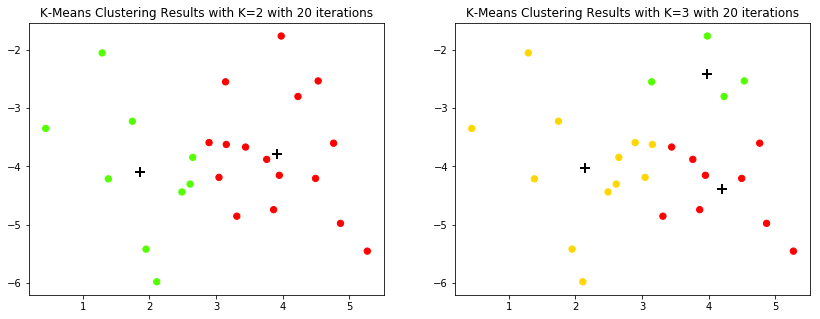
\includegraphics[width=0.7\textwidth]{clusteringMethods/kmeansclustering/fig/k-mean.png}
	\caption{K-Means Clustering Results with K=2 with 20 iterations on the right and  with K=3 with 20 iterations on the left}
	\label{fig:kmeansclusteringk2_20Iteration}
\end{figure}

While k-means clustering is a good algorithm, it is not without it's own flaws. When running K-means clustering with a large number of iterations, such as 20 since otherwise an undesirable local optimum may be obtained. Which simply means that, more than one run of the algorithm with randomized starting centroids could give a better result.




\section{Hierarchical clustering}

With K-means clustering we had to predefine the number of clusters $K$. This can be a disadvantage, since we would have to do some initial analysis of the data prior to clustering it. Hierarchical clustering does not require this predefinition. It uses a bottom-up tree algorithm or agglomerative approach to build a dendrogram starting from the observation leaves and ends up combining this into clusters at the trunk. This gives us a flexibility in the number of clusters.

\subsection{Theory}

Agglomerative states that each observation starts in its own cluster and with each iteration of the process are paired with other clusters as we move up the hierarchy.  This is based on a \textit{metric} criteria, a measure of distance between the pairs, and a \textit{linkage} criteria that indicate the dissimilarity between pairwise sets.

A common metric is the Euclidean distance:
\begin{align}
	d(a,b) = \sqrt{\sum (a_{i} - b_{i})^{2}}  %TODO Christian did you done goof in equation 7.4? with the underlined 2
\end{align}

Which is the straight-line distance between two points in Euclidean space (\textit{n}-space with \textit{n}-tuples of real numbers). Between two points \textit{a} and \textit{b} given by ($X_a$, $Y_a$) and ($X_b$, $Y_b$) the Euclidean distance d(a,b) is:
\begin{align}
	d(a,b) = \sqrt{(X_a - X_b)^2 + (Y_a - Y_b)^2}
\end{align}

Linkage determines which distances to use between sets of observations, i.e. how they are grouped together. \textit{Single} minimizes the distance between the closest elements in clusters, \textit{complete} maximizes distance between the farthest elements, \textit{average} finds the mean of all pairwise distances, and \textit{ward} joins clusters based on the total distance between their centroids. Figure \ref{fig:linkagecriteria} shows the three kinds of linkages to calculate distance.

\begin{figure}[H]
	\centering
	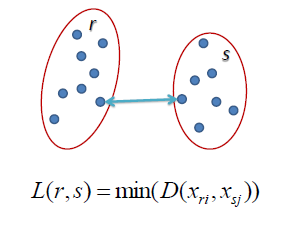
\includegraphics[width=0.3\textwidth]{clusteringMethods/hierarchicalclustering/fig/ClusteringSingle.png}
	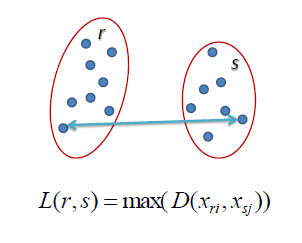
\includegraphics[width=0.3\textwidth]{clusteringMethods/hierarchicalclustering/fig/ClusteringComplete.png}
	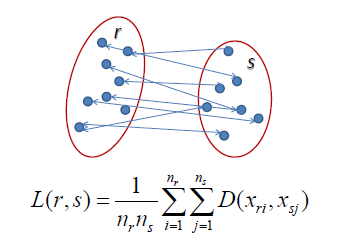
\includegraphics[width=0.3\textwidth]{clusteringMethods/hierarchicalclustering/fig/ClusteringAverage.png}
	\caption{The single, complete and average linkage criteria.}
	\label{fig:linkagecriteria}
\end{figure}

The algorithmic steps for hierarchical clustering are:

1. Start with \textit{N} clusters, one for each data point. \\
2. Merge the clusters that are closest to each other. This gives \textit{N-1} clusters. \\
3. Calculate the distance between the clusters using a linkage criteria (complete, single etc.) \\
4. Repeat step 2 and 3 until we end up with one cluster with \textit{N} data points. The end result is a dendrogram picturing the distance (clusters) as a function of the observations (labels).

\subsection{Results}
\subsubsection*{LAB 10.5.2}%TODO rewise exercise
Lab 10.5.2 is using hierarchical clustering to group a 50 x 50 matrix of random observations using Euclidean distance and complete linkage in to two clusters. The AgglomerativeClustering package from Sklearn provides agglomerative clustering functionality in Python to recursively merge pairs of clusters.The Agglomerative Clustering gives the following output.

\noindent\textit{Labels:[1 0 1 1 0 0 0 0 0 0 1 0 0 0 1 0 0 1 10]}

\noindent\textit{No. leaves:  20}

\noindent\textit{No. clusters:  2}


\noindent labels from the complete agglomerative clustering process show how the observations are grouped, starting from $X_i$ to $X_n$. A label [0 1 1 1 0] says observation $X_0$ belongs to the first final cluster, $X_1$ to the second final cluster, $X_2$ to the second etc. The number of leaves correspond to the observations points ($X_a$, $Y_a$). We then generate a dendrogram to picture the Euclidean distance between clusters and their labels. Figure \ref{fig:dendrogramcluster} shows the dendrograms of the three performed clusterings.

\begin{figure}[H]
	\centering
	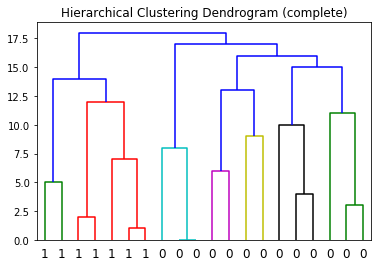
\includegraphics[width=0.3\textwidth]{clusteringMethods/hierarchicalclustering/fig/CompleteClustering.png}
	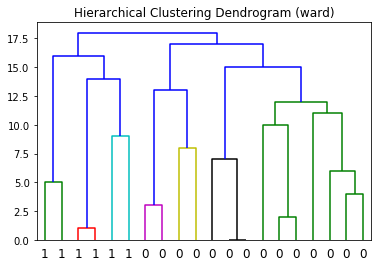
\includegraphics[width=0.3\textwidth]{clusteringMethods/hierarchicalclustering/fig/WardClustering.png}
	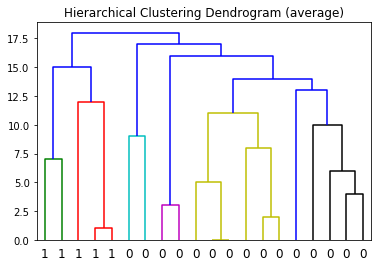
\includegraphics[width=0.3\textwidth]{clusteringMethods/hierarchicalclustering/fig/AverageClustering.png}
	\caption{Dendrograms for complete, ward and average clustering.}
	\label{fig:dendrogramcluster}
\end{figure}

\noindent Also in Figure \ref{fig:dendrogramcluster} is sowing that hierarchical clustering correctly identifies the lower left cluster and the lower right one, however with ward and average a significant euclidean distance has to be reached for it to split correctly, whereas complete splits the observations into two separate ones early on. 

%TODO What is a ward Christian?








						\clearpage
\chapter{Discussion} \label{ch:discussion}								        \clearpage
\chapter{Conclusion} \label{ch:conclussion}
Throughout this report we have discussed various methods for implementing statistical concepts for supervised and unsupervised learning, in decision support systems. We have used real data from football players in the NFL and housing prices in Boston to compute linear regression models that can predict future outcome. We found improvements to the training part of regular regression by applying discriminant analysis and to the test part with re-sampling methods to enhance the model accuracy. Subset selections and shrinkage methods cover the same concept of creating models based on predictors. We have studied different ways of validating models and learned the strengths of using the mathematically simple cross validation. We have used K-means and unsupervised learning to find clusters, within given datasets.

In the report we describe the fundamentals of statistical models used in machine learning and have acquired the basic knowledge of how to apply them in a real-life context.										\clearpage
\chapter{Perspectives} \label{ch:perspectives}									\clearpage
\bibliographystyle{plainnat}
\bibliography{bibliography/mendeley/DecisionSupportSystems} \label{ch:bibliography}
									\clearpage

%etc...

\end{document}
